\documentclass{zah}

\title{Návrh systému evidencie plynových fliaš}
\author{Oliver Laštík, Šimon Strieška, Jozef Špirka, Adam Zahradník}

\begin{document}
\maketitle

\tableofcontents
\cleardoublepage

\section{Špecifikácia vonkajších interfejsov}

Systém beží na webovom serveri, ku ktorému používateľ pristupuje cez webový prehliadač. Webový server poskytuje užívateľovi prístup k funkcionalitám systému prostredníctvom HTTPS protokolu. Systém uchováva informácie o plynových fľašiach a používateľoch v databáze. Na komunikáciu s databázou využíva framework Django. Databázové dotazy sú zasielané na server cez SQL protokol. Systém komunikuje s používateľom prostredníctvom grafického rozhrania (GUI) vo webovom prehliadači. GUI poskytuje užívateľovi možnosť nahrávať fotografie manometra, zobrazovať, pridávať, mazať, upravovať a exportovať údaje o plynových fľašiach. Pri pokuse o detekciu manometra systém komunikuje s kamerou daného zariadenia. Pri prvom pokuse o detekciu manometra si systém vyžiada povolenie od používateľa na používanie kamery. Interakcia s kamerou prebieha cez natívne API pre kamery v danom zariadení.

\section{Dátový model}
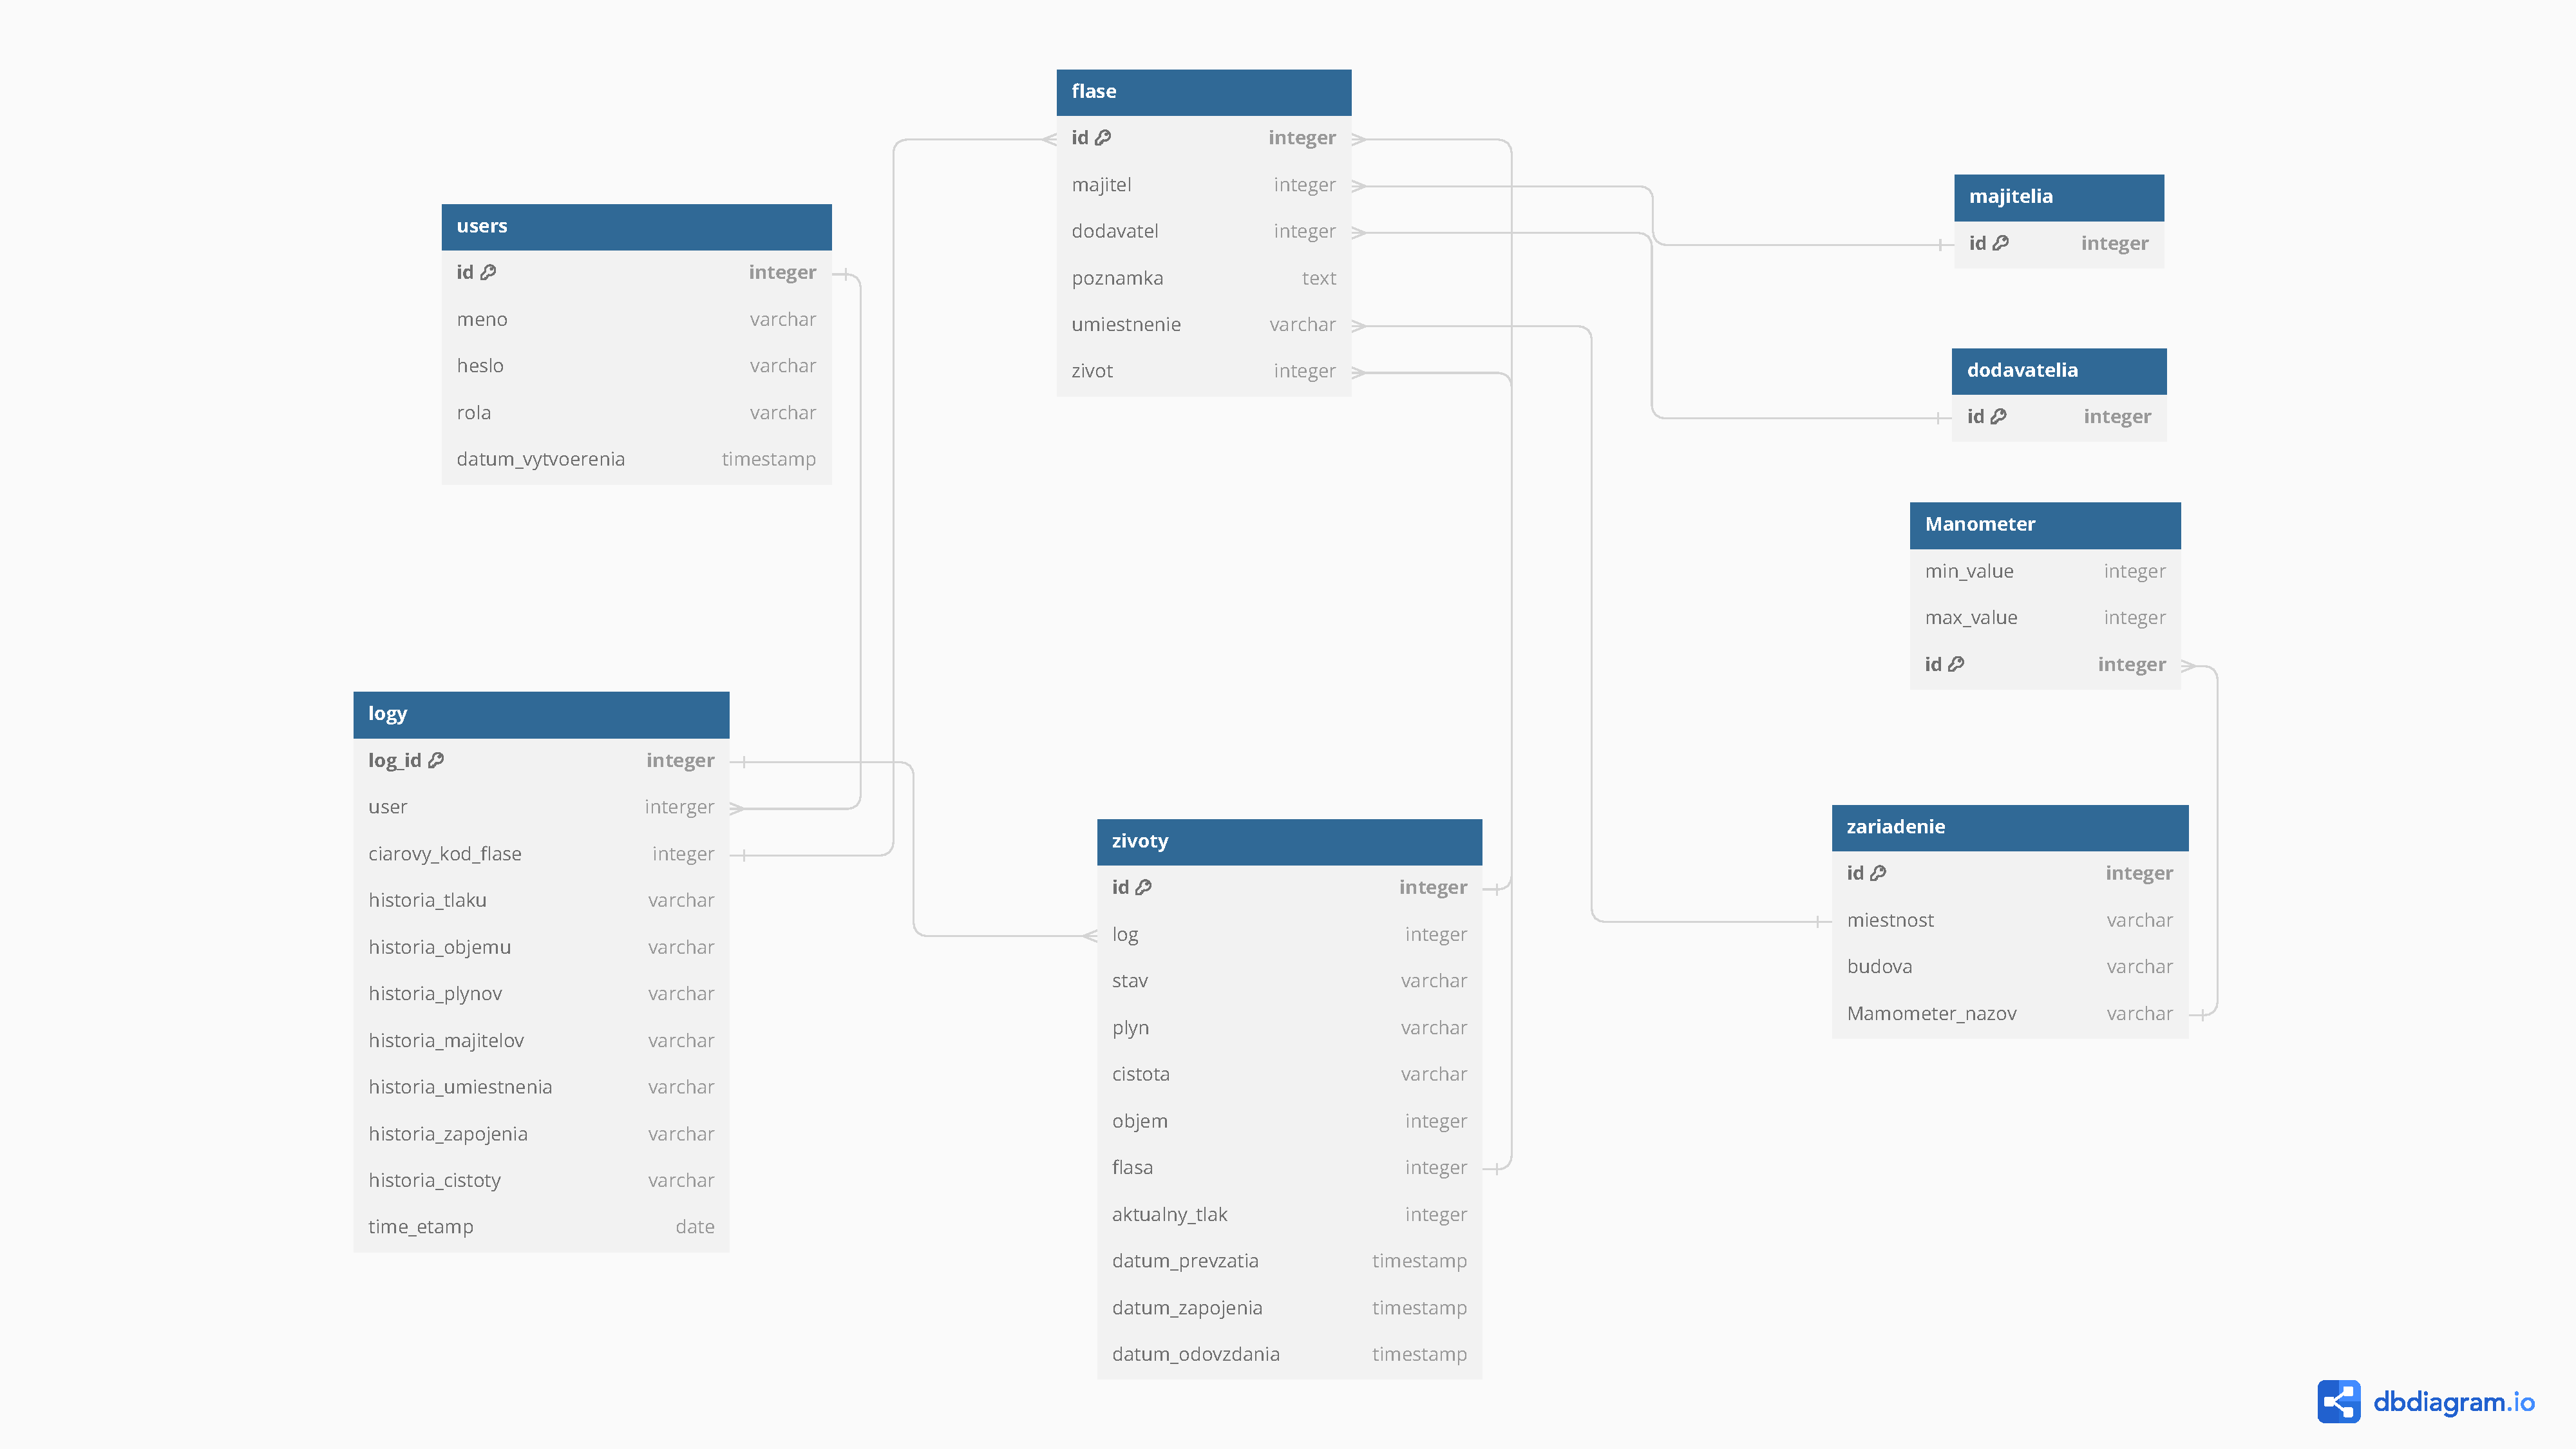
\includegraphics[width=\textwidth]{navrh-assets/db}

Databáza sa skladá z viacerých tabuliek, ktoré sú navzájom prepojené cez cudzie kľúče. Hlavné tabuľky zahŕňajú:

\begin{itemize}
    \item \textbf{flase\_app\_user}: Obsahuje informácie o používateľoch systému vrátane ich rolí a autentifikačných údajov.
    \item \textbf{flase\_app\_cylinder}: Uchováva záznamy o jednotlivých fľašiach, ich umiestnení, vlastníkoch a životných cykloch.
    \item \textbf{flase\_app\_cylinderlife}: Zaznamenáva rôzne stavy fľaši, vrátane údajov o tlaku, plyne a objeme.
    \item \textbf{flase\_app\_cylinderchange}: Uchováva logy súvisiace s operáciami a udalosťami týkajúcimi sa fľaši.
    \item \textbf{flase\_app\_supplier}, \textbf{flase\_app\_gas}, \textbf{flase\_app\_owner}, \textbf{flase\_app\_location}, \textbf{flase\_app\_workplace},\textbf{flase\_app\_building}: Tieto tabuľky poskytujú dodatočné informácie o dodávateľoch, vlastníkoch, plynoch, umiestneniach, pracovnom prostredi a budove spojených s fľašami.
\end{itemize}

Každá tabuľka je navrhnutá s cieľom optimalizovať ukladanie a prístup k dátam potrebným pre správu a sledovanie fľaši a súvisiacich aktivít.

\subsection{State diagram}
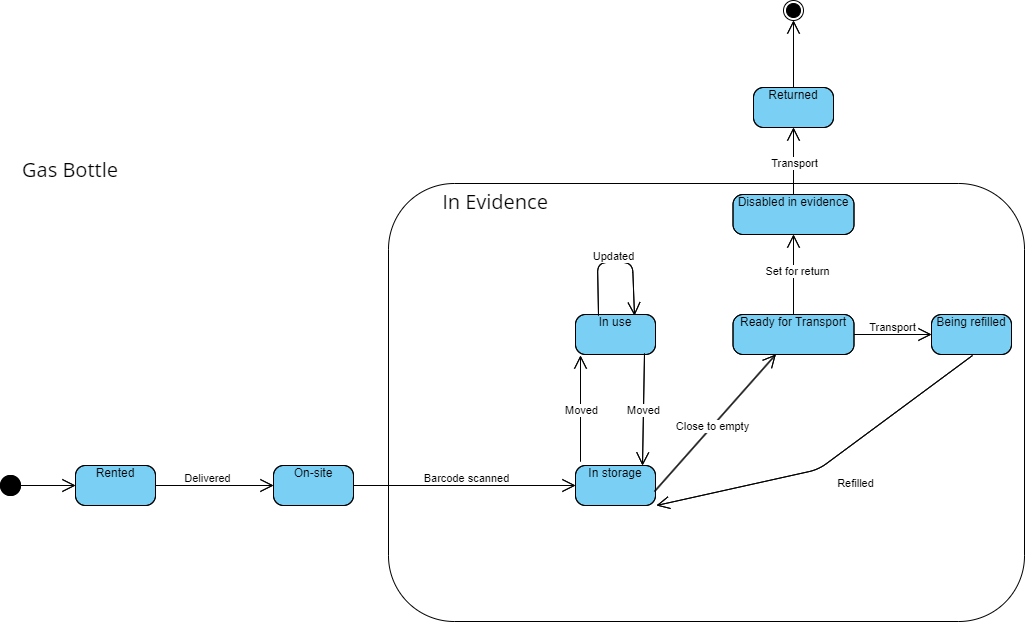
\includegraphics[width=\textwidth]{navrh-assets/state}

\section{Návrh používateľského rozhrania}

\subsection{Prihlasovacia obrazovka}
\begin{center}
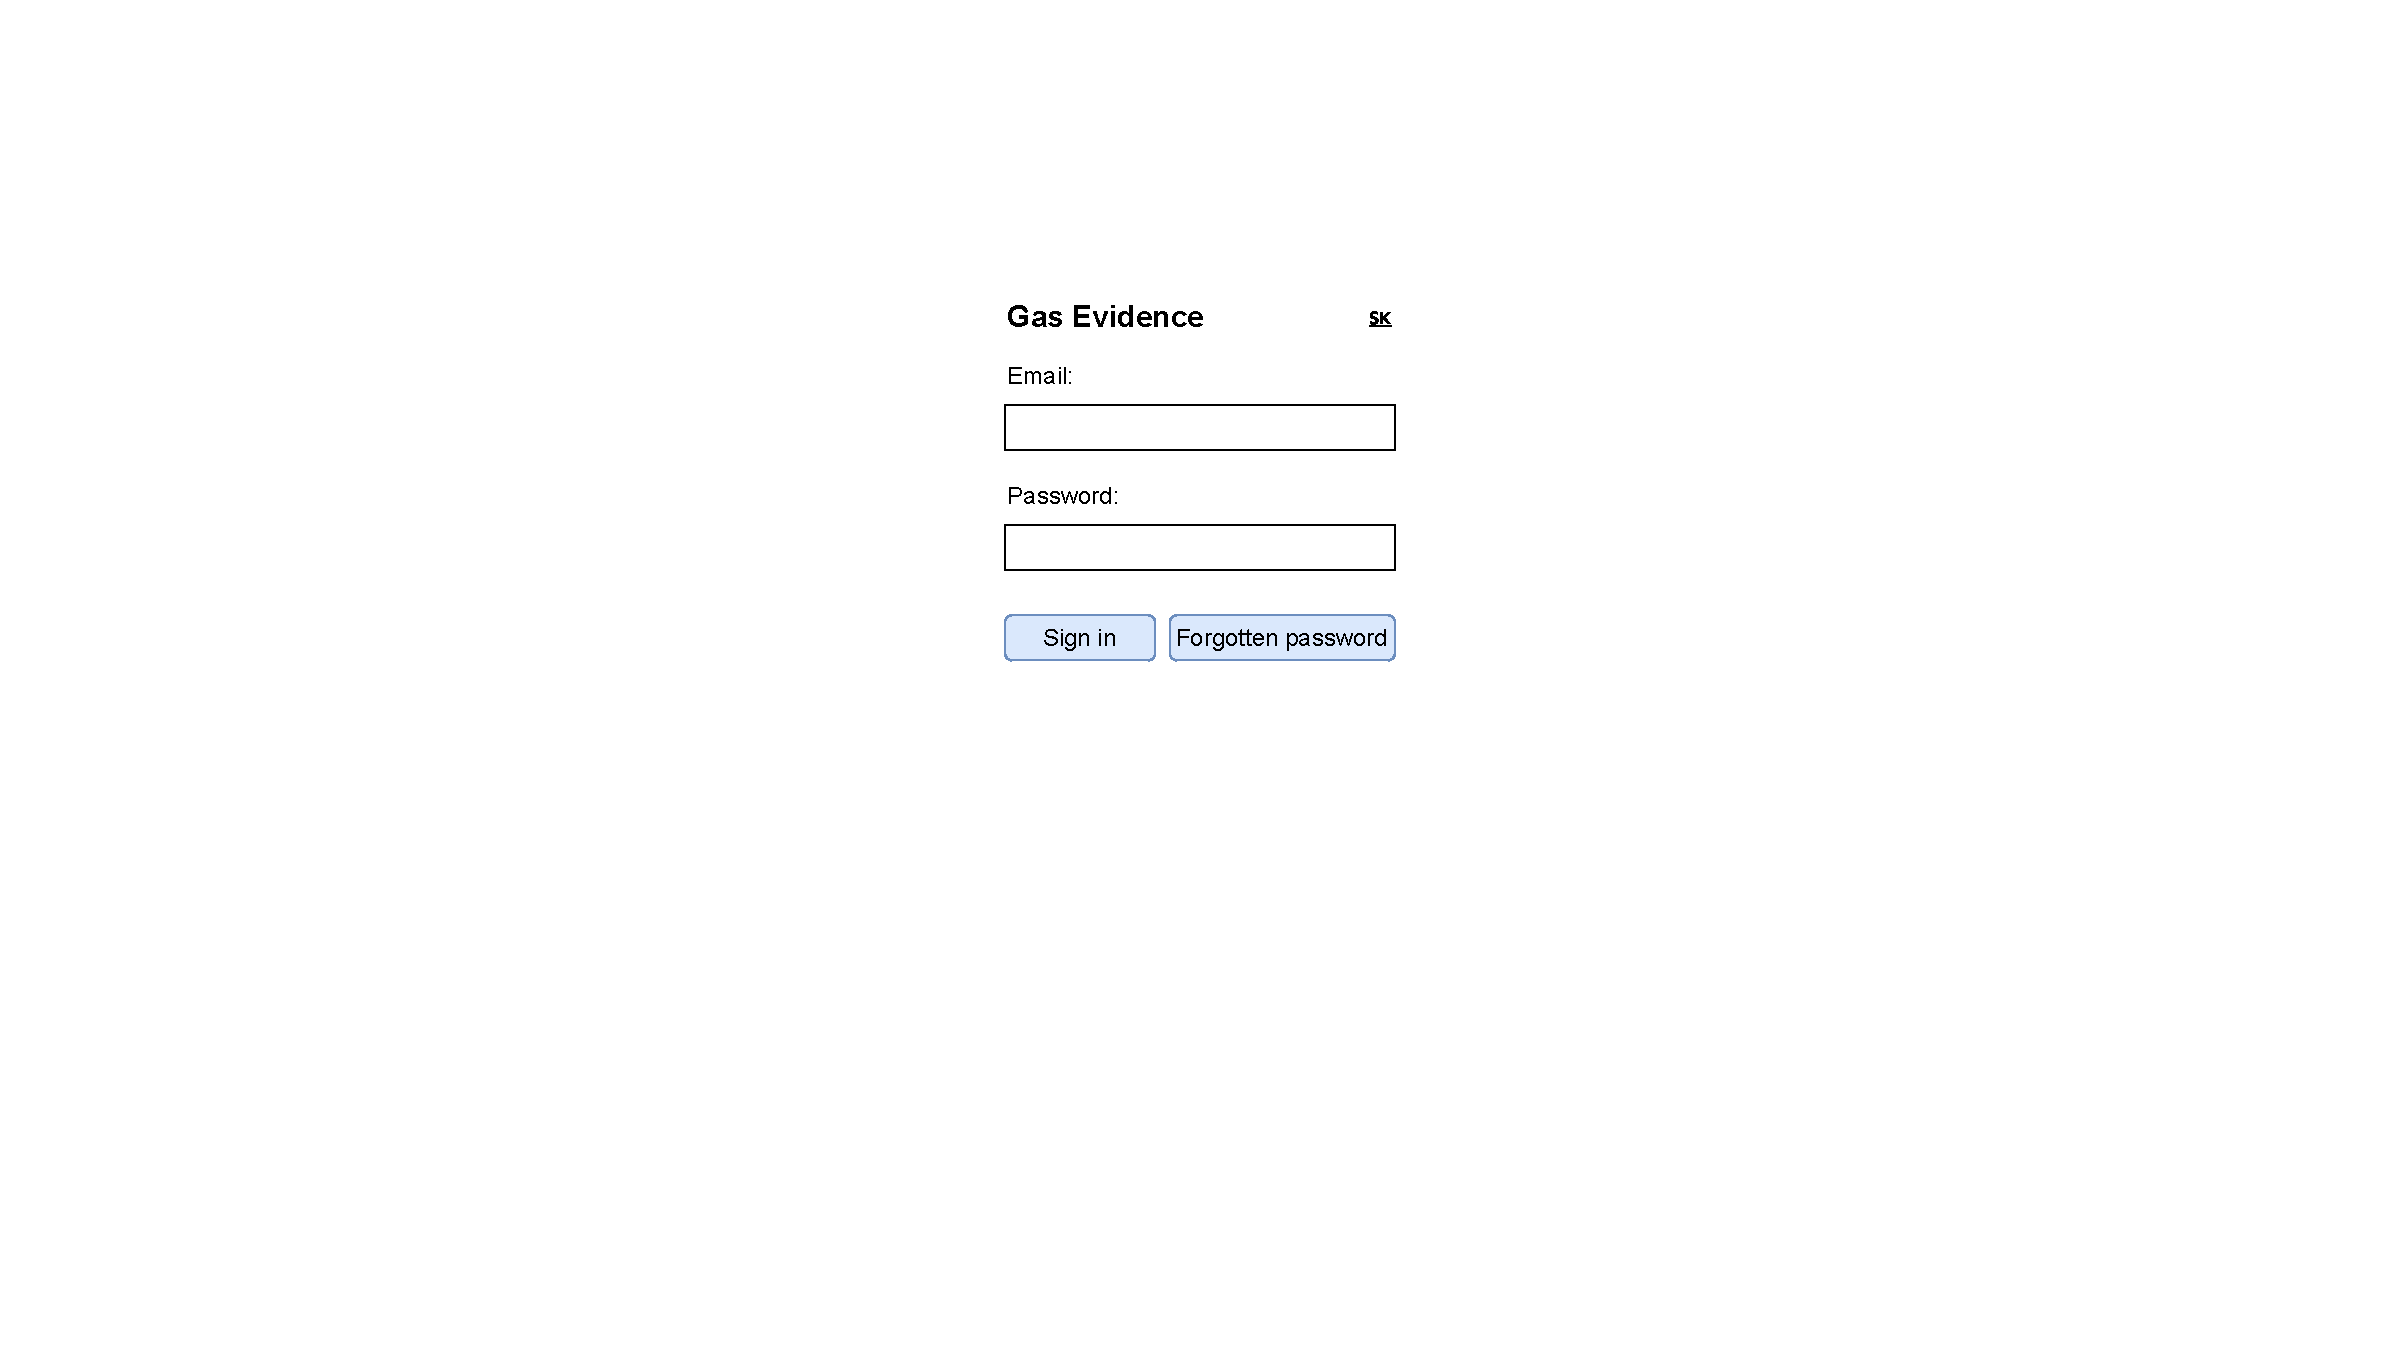
\includegraphics[width=.7\textwidth,page=1]{navrh-assets/ui}
\end{center}

\subsection{Navigačné menu}
\begin{center}
\includegraphics[width=.7\textwidth,page=2]{navrh-assets/ui}
\end{center}

\subsection{Zoznam fliaš}
\begin{center}
\includegraphics[width=.7\textwidth,page=3]{navrh-assets/ui}
\end{center}

Na mobilnom zariadení sa miesto tabuľky zobrazí vertikálny zoznam.

\subsection{Detail fľaše}
\begin{center}
\includegraphics[width=.7\textwidth,page=4]{navrh-assets/ui}
\end{center}

\subsection{Úprava fľaše}
\begin{center}
\includegraphics[width=.7\textwidth,page=5]{navrh-assets/ui}
\end{center}

\subsection{Pridanie fľaše}
\begin{center}
\includegraphics[width=.7\textwidth,page=6]{navrh-assets/ui}
\end{center}


\subsection{Zoznam dodávateľov}
\begin{center}
\includegraphics[width=.7\textwidth,page=7]{navrh-assets/ui}
\end{center}
Analogicky pre majiteľov a plyny.

\subsection{Pridanie/úprava dodávateľov}
\begin{center}
\includegraphics[width=.7\textwidth,page=8]{navrh-assets/ui}
\end{center}
Analogicky pre majiteľov a plyny.

\subsection{Zoznam používateľov}
\begin{center}
\includegraphics[width=.7\textwidth,page=9]{navrh-assets/ui}
\end{center}

\subsection{Pridávanie/úprava používateľov}
\begin{center}
\includegraphics[width=.7\textwidth,page=10]{navrh-assets/ui}
\end{center}

\subsection{Fotenie manometra}
\begin{center}
\includegraphics[width=.7\textwidth,page=11]{navrh-assets/ui}
\end{center}
Na pravo výsledok merania, dá sa ručne upraviť v prípade zlej detekcie.

\section{Návrh implementácie}

\subsection{Component diagram}
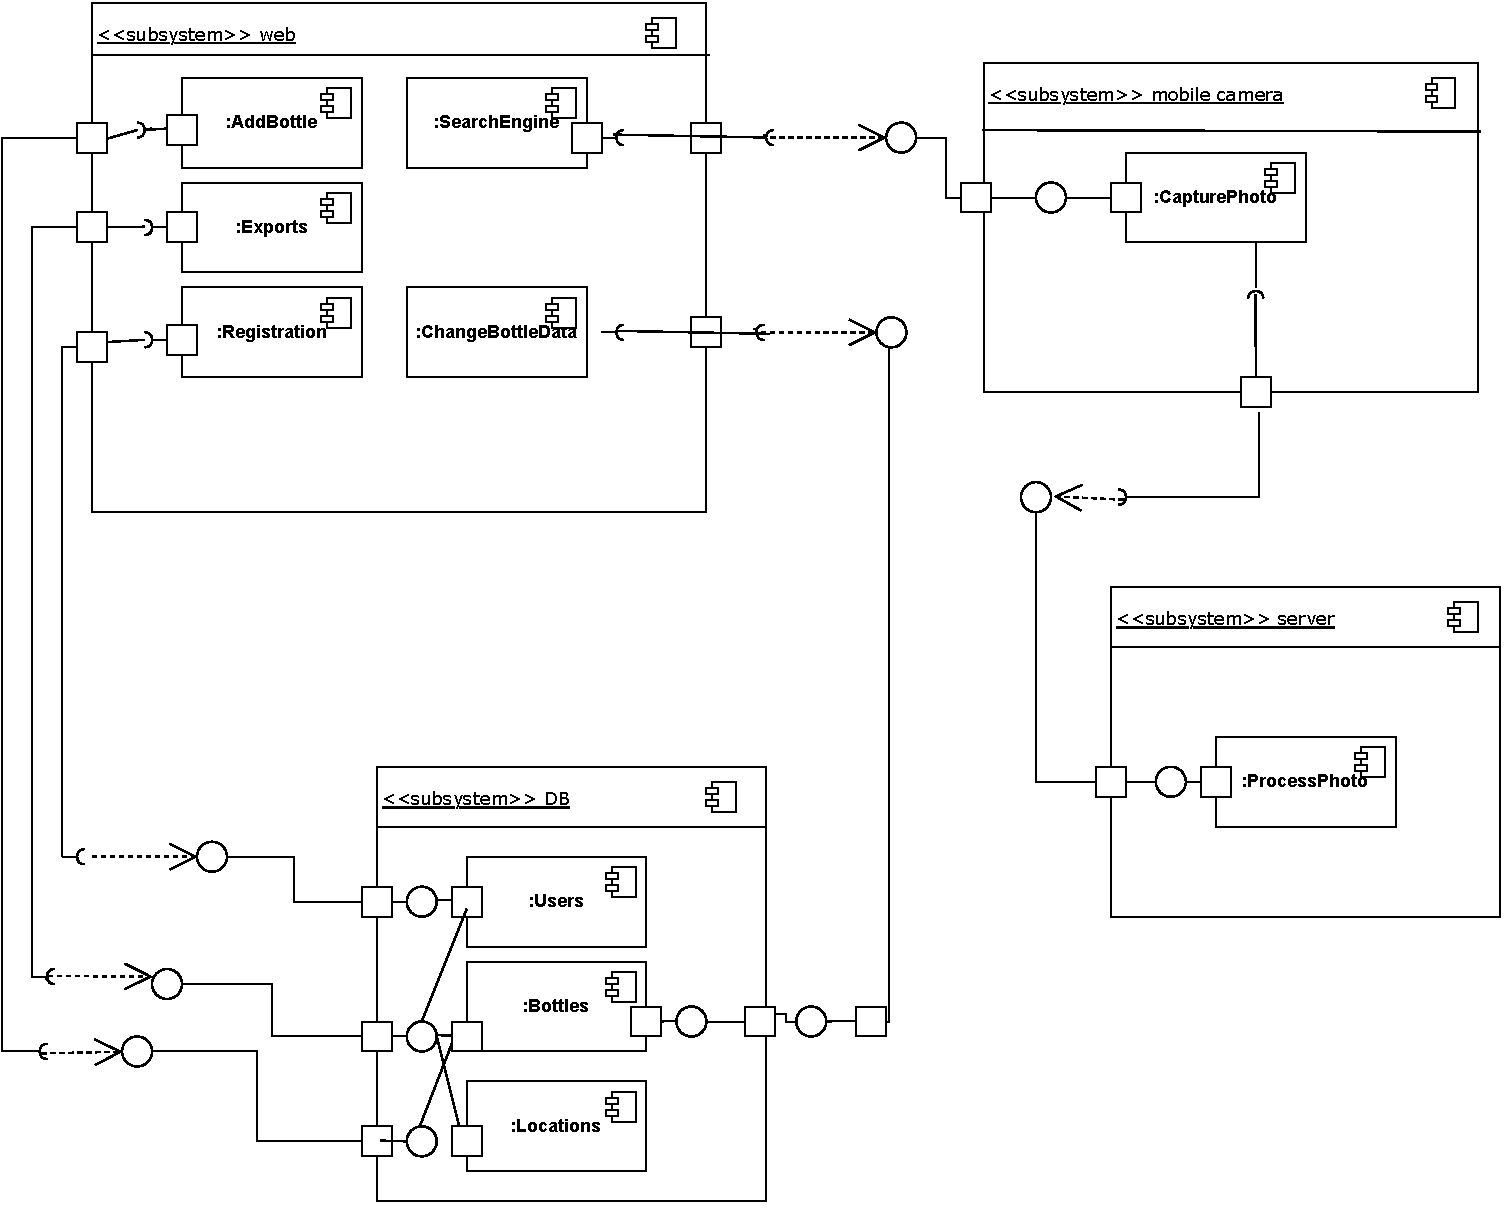
\includegraphics[width=\textwidth]{navrh-assets/component}

\section{Deployment}
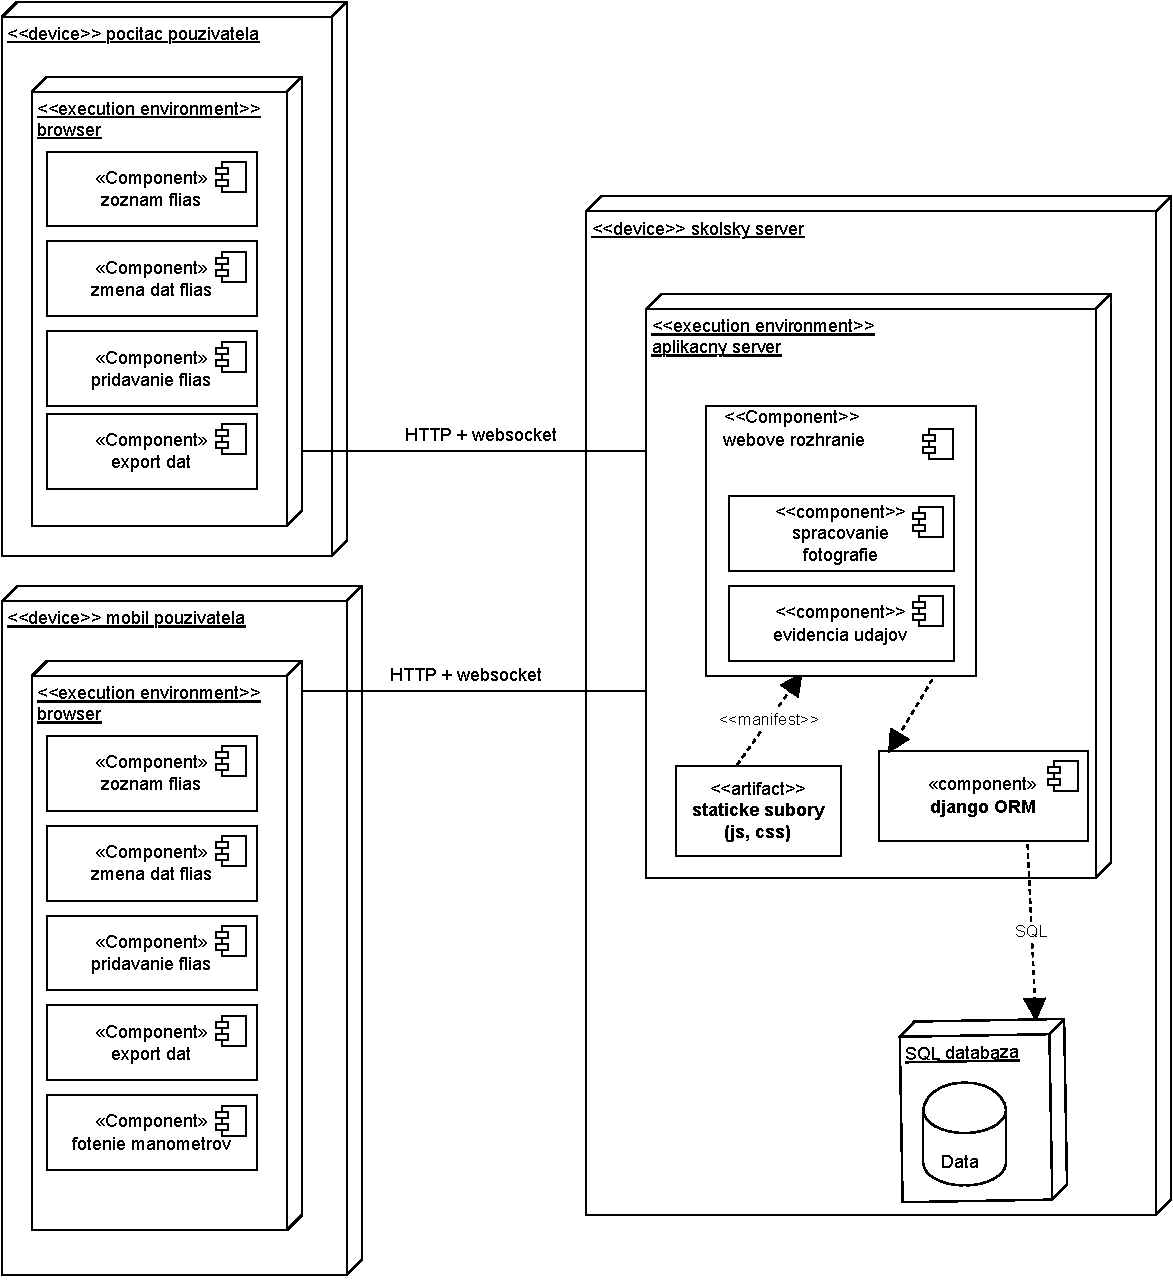
\includegraphics[width=\textwidth]{navrh-assets/deployment}

\section{Použité technológie}

Pri realizácií projektu sme sa rozhodli použiť nasledujúce webové technológie:

\begin{itemize}
\item Python: primárny programovací jazyk
\item Django: framework na vývoj webových aplikácií v Pythone
\item Bootstrap: CSS framework
\item HTML, JS, CSS
\item OpenCV: nástroj počítačového videnia
\item NumPy: nástroj matematických výpočtov v Pythone
\item PostgreSQL / SQLite3: relačný databázový systém
\end{itemize}

\section{Plán implementácie}

\begin{enumerate}
	\item Prihlasovanie používateľov
	\item Zoznam a správa majiteľov
	\item Zoznam a správa dodávateľov
	\item Zoznam a správa plynov
	\item Zoznam a správa používateľov
	\item Zoznam fliaš
	\item Vyhľadávanie fliaš
	\item Filtrovanie fliaš
	\item Príjem nových fliaš
	\item Menenie parametrov fľaše
	\item Zobrazovanie histórie fliaš
	\item Manuálne zadávanie tlaku
	\item Export dát
	\item Automatické rozoznávanie tlaku
\end{enumerate}

\end{document}
